\subsubsection{Multiple Comparisons}
While t-test allows for the testing for cohesion between two mean values, it can often be insufficient when trying to calculate mean values of multiple test statistics. If more than two mean values are to be calculated, it must be done with pairwise testing. Every test increases the risk of committing type 1 errors i.e. accidentally rejecting a hypothesis that is actually true. Given a 5\% level of significance, the risk is thus 5\% per test. Therefore, if five mean values are to be tested (m1=m2=m3=m4=m5), the number of required tests would be 10, because all combinations must be executed. The combinatory conditions are calculated as follows:

\begin{equation}
\binom{n}{m} = {\frac{n!}{(m(m-n)!)}} 
\end{equation}\\
Meaning we will have the following amount of combinations:

\begin{equation}
\binom{5}{2} = {\frac{5!}{(2(5-2)!)}} = 10 
\end{equation}\\
This entails that every combination increases the uncertainty of type 1 errors, and that the aggregated probability that at least one type 1 error will not be present in one of the tests is:

\begin{equation}
1-0,95^{10}= 0,598 = 59,8\%
\end{equation}\\
Hence, the probability  that at least one type 1 error will be present is approximately 40,2\%. The risk of committing a type 1 error will thus, increase explosively when the t-test is applied to mean-value comparisons of more than two populations.
\\

\subsubsection{Analysis of Variance (ANOVA)}
This increased risk can be very damaging for the credibility of any test; therefore it may be beneficial to eliminate as many confounding factors as possible. An \textit{analysis of variance}-test (ANOVA) may advantageously be used, as it is capable of comparing several mean values at once, and computing the variance.  To use ANOVA, one must apply the variance within each population as well as the variance between the populations. The formula for the 1-way ANOVA-test, also referred to as F-test, can thus be written:

\[F=\frac{between-group-variables}{within-group-variables}\]

Thereby testing the mean value simultaneously rather than pairwise.
In the exercise (\textit{Design and Analysis of Experiments V: Exercies} by Sofia Dahl) three painkillers have to be compared to each other along with a placebo-version. Hence, there are four mean values that must be compared.  Instead of using the painkiller-data, we will analyse the data acquired by the 10th Semester group with a multiple comparison of means using the ANOVA-test, just like we have done in the previous assignments.
Since there are quite many dimensions of the aforementioned dataset, it is necessary to restrict ourselves to a few examples. An entire review of the dataset could easily fill an entire report.
It is appropriate both logically and feasibly to start out with expanding the tests from exercice 1.2 and 1.3 to also include \textit{intellectual engagement for Mouse and Keyboard} after 15 minutes, and \textit{Physical engagement} for Head Mounted Display (HMD) after 30 minutes. Thus we have added an extra mean value that must be testet in the two tests, therefore we will use the one-way analysis of variance (ANOVA1).\\


\begin{figure}[t]
	\centering
	\begin{subfigure}[t]{0.48\textwidth}
		\includegraphics[width=\textwidth]{fig/{intellectualMK_testvalue}.png}
		\caption{Statistics}
		\label{IntellectMKtestVal}
	\end{subfigure}
	\begin{subfigure}[t]{0.48\textwidth}
		\includegraphics[width=\textwidth]{fig/{intellectualMK}.png}
		\caption{Boxplot}
		\label{intellectMK}
	\end{subfigure}
	
	\caption{XX EXPLANATION XX}
	\label{ANOVA_1}
\end{figure}

Similar tests can be performed for all seven formats of engagement included in the data. But as mentioned previously, such a review would be comprehensive. If all combinations were to be tested we would have to test all of the three methods (MK, Wii and HMD) seven times, as well as seven times for each of the three time-entries (5,15 and 30) which would aggregate a total of 42 tests.

\begin{figure}[t]
	\centering
	\begin{subfigure}[t]{0.48\textwidth}
		\includegraphics[width=\textwidth]{fig/{physical_testvalue}.png}
		\caption{Statistics}
		\label{PhysicalMKtestVal}
	\end{subfigure}
	\begin{subfigure}[t]{0.48\textwidth}
		\includegraphics[width=\textwidth]{fig/{physical}.png}
		\caption{Boxplot}
		\label{PhysicaltMK}
	\end{subfigure}
	
	\caption{XX EXPLANATION XX}
	\label{ANOVA_1.1}
\end{figure}

ANOVA kan dog også anvendes til at inkludere endnu en dimension. Hvis vi fx vil teste intellectual engagement for de tre metoder i hver af de tre tidsangivelser. Dermed har vi en dimension af både metode og tid. Hertil skal anvendes ANOVA 2, som tester, om der er forskel på middelværdierne i de to dimensioner samtidig.

\begin{figure}[t]
	\begin{center}
		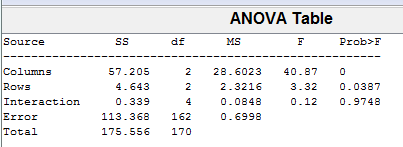
\includegraphics[height=5cm]{fig/anova2_testvalue.png}
		\caption{XX EXPLANATION XX}
		\label{ANOVA_2}
	\end{center}
\end{figure}

